\documentclass[12pt]{article}

\usepackage{fullpage}
\usepackage{multicol,multirow}
\usepackage{tabularx}
\usepackage{listings}
\usepackage{pgfplots}
\usepackage[utf8]{inputenc}
\usepackage[russian]{babel}
\usepackage{pgfplots}
\usepackage{tikz}

% Оригиналный шаблон: http://k806.ru/dalabs/da-report-template-2012.tex

\begin{document}

\section*{Лабораторная работа №5\, по курсу дискрeтного анализа: Суффиксные деревья}

Выполнил студент группы М8О-312Б-22 МАИ \textit{Юрков Евгений}.

\subsection*{Условие}

\textbf{Вариант:} 5

Найти самую длинную общую подстроку двух строк с использованием суффиксного дерева.

\textbf{Формат ввода:}
Две строки.

\textbf{Формат вывода:}
На первой строке нужно распечатать длину максимальной общей подстроки,
затем перечислить все возможные варианты общих подстрок этой длины
в порядке лексикографического возрастания без повторов.

\newpage
\subsection*{Метод решения}

Для построения суффиксного дерева за линейное время был использован алгорим Укконена.
Чтобы найти самую длинную общую подстроку необходимо было построить обобщенное суффиксное дерево,
для этого в каждой вершине хранятся номера строк, которые содержат данный суффикс.
Поиск осуществляется по следующему принципу: обходом в глубину находятся все подстроки вершин,
которые принадлежат сразу всем строкам и выбирается самая длинная.
Данный алгоритм может также использоваться для поиска максимальной общей подстроки 
более чем двух строк.

% \newpage
\subsection*{Описание программы}

Все алгоритмы реализованы в классе \texttt{SuffTree}, содержащем следующие методы:
\begin{itemize}
    \item \texttt{SuffTree} - конструктор, строящий дерево из одной или нескольких строк;
    \item \texttt{add} - метод дополняющий обобщенное суффиксное дерево ещё одной строкой;
    \item \texttt{max\_com\_substr} - поиск самой длинной общей подстроки для всех строк,
                                    содержащихся в дереве;
    \item \texttt{Print} - вывод структуры дерева, для удобной отладки;
\end{itemize}

%\newpage
\subsection*{Дневник отладки}

\begin{enumerate}
    \item исправлено создание суффиксных ссылок, чтобы они не указывали на корень
    \item исправлено разделение вершины, чтобы вершины, имеющие ссылку на неё, не теряли её
    \item добавлена проверка и исправление массива, указывающего на то, к какой строке относится вершина,
          так как из за перехода по ссылкам не все вершины отмечали свои строки.
\end{enumerate}

\newpage
\subsection*{Тест производительности}

Алгоритм Укконена для построения суффиксного дерева работает за линейное время: $O(n)$, где $n$ -- длина строки.
\begin{figure}
    \centering
    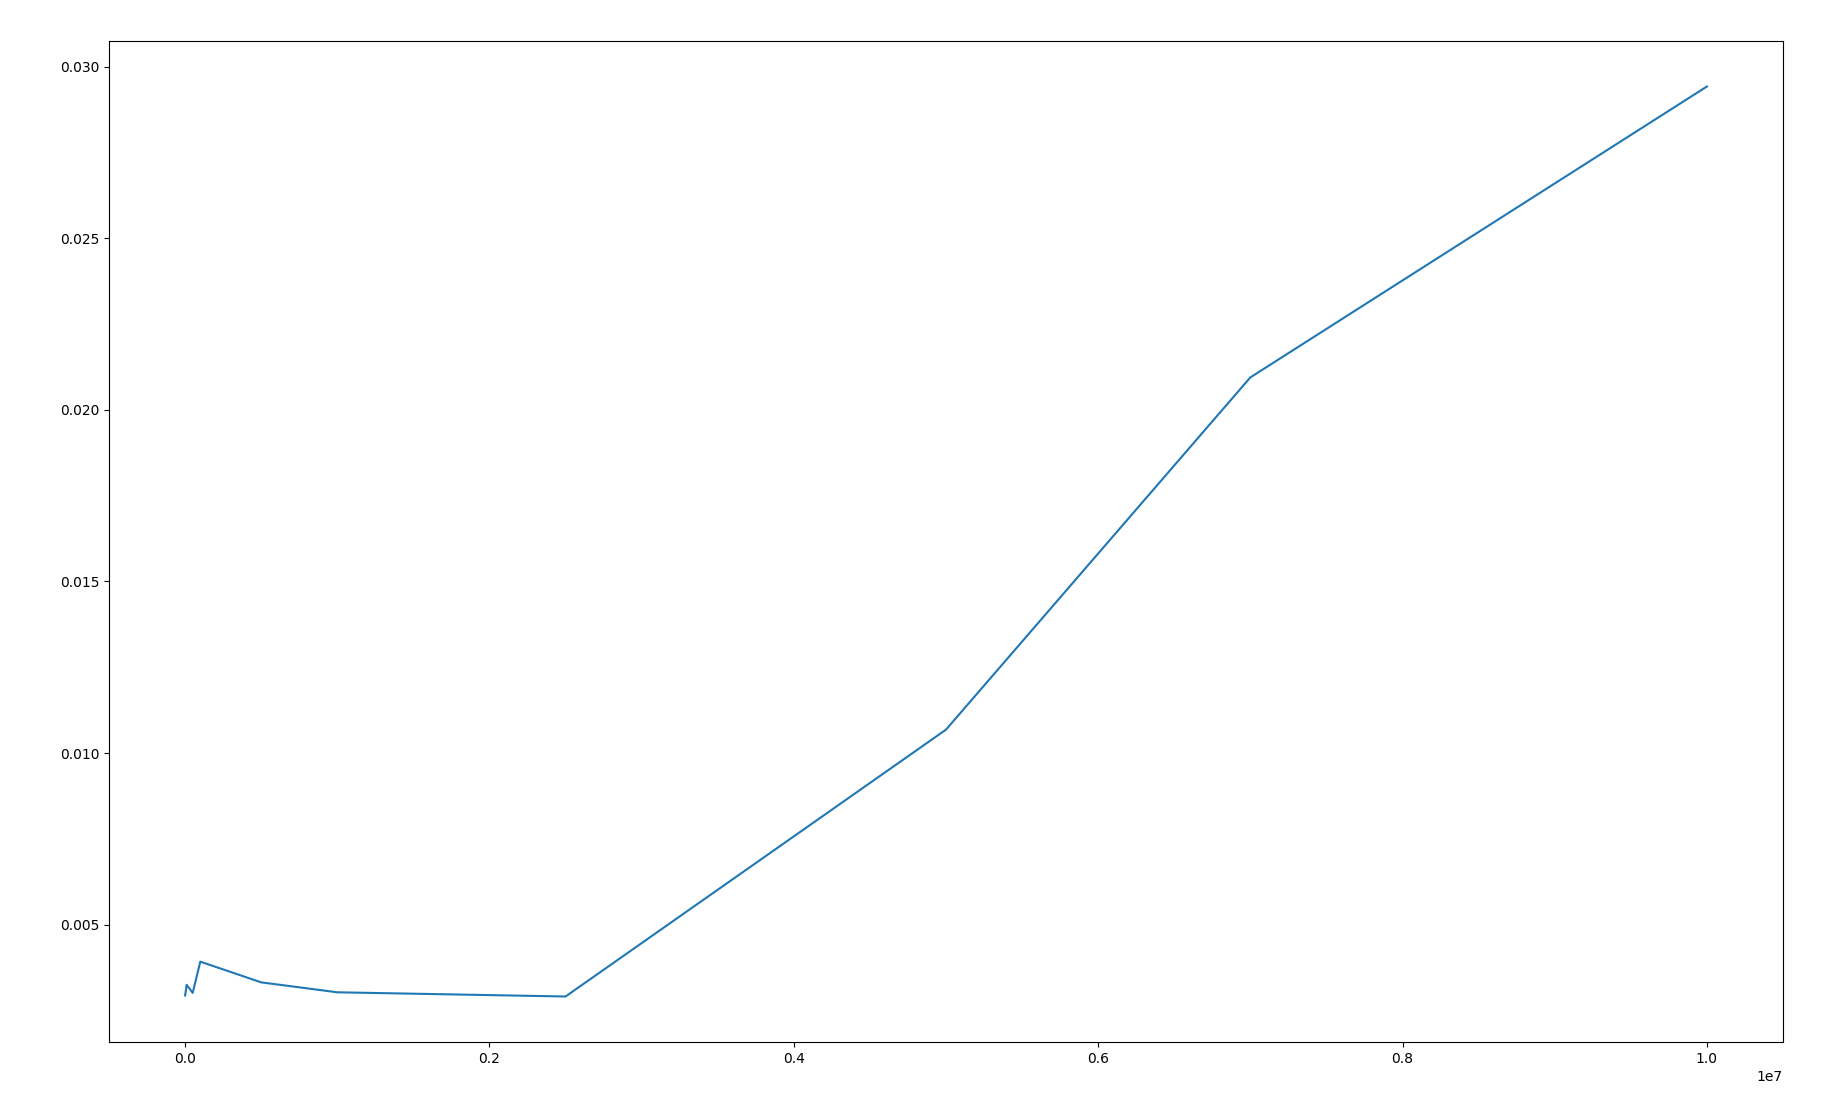
\includegraphics[width=\textwidth]{graph.png}
    \caption{График зависимости времени работы программы от длины строки}
\end{figure}

\newpage
\subsection*{Выводы}

В ходе данной лабораторной работы была реализована программа,
предназначенная для поиска самой длинной общей подстроки двух строк
с помощью суффиксного дерева. Алгоритм Укконена для построения
суффиксного дерева работает за линейное время $O(n)$, в отличие от наивного,
который работает за $O(n^3)$.
Для поиска максимальной общей подстроки было применено
обобщенное суффиксное дерево для двух строк,
что позволило эффективно решать задачу.

Суффиксные деревья очень полезны в анализе текстов и поисковых задачах.
Они применяются для эффективного поиска подстрок,
сжатия данных, а также для построения суффиксных массивов.
Их важность заключается в способности
быстро находить различные паттерны в строках, обеспечивая высокую
производительность даже при больших объемах данных.

Несмотря на свою скорость, суффиксные деревья занимают большое количество
памяти, поэтому в случаях, где память важнее используют суффиксные массивы.
Суффиксные массивы работают дольше, но занимают гораздо меньше памяти.

\end{document}